\documentclass[aspectratio=169,12pt]{beamer}

% Build from the repository root: make lecture-03-slides
\usepackage[T1]{fontenc}
\usepackage{lmodern}
\usepackage{amsmath,amssymb,booktabs,array}
\usepackage{pgfplots}
\usepgfplotslibrary{groupplots}
\pgfplotsset{compat=1.18}
\usefonttheme{professionalfonts}

\definecolor{Ink}{HTML}{16324F}
\definecolor{Blue}{HTML}{1F4E79}
\definecolor{Orange}{HTML}{C46A13}
\definecolor{Teal}{HTML}{007D80}
\definecolor{Muted}{HTML}{526477}
\setbeamercolor{normal text}{fg=Ink,bg=white}
\setbeamercolor{frametitle}{fg=Ink}
\setbeamercolor{structure}{fg=Blue}
\setbeamercolor{footline}{fg=Muted}
\setbeamerfont{frametitle}{size=\large,series=\bfseries}
\setbeamerfont{footline}{size=\tiny}
\setbeamersize{text margin left=8mm,text margin right=8mm}
\setbeamertemplate{navigation symbols}{}
\setbeamertemplate{headline}{}
\setbeamertemplate{frametitle}{%
  \vspace{3mm}\insertframetitle\par\vspace{1mm}}
\newcommand{\conspectsection}{3.1}
\setbeamertemplate{footline}{%
  \hspace{8mm}\usebeamerfont{footline}\usebeamercolor[fg]{footline}%
  Conspect \S\,\conspectsection\hfill\insertframenumber\hspace{8mm}\vspace{3mm}}
\setlength{\parskip}{0.5em}
\setlength{\abovedisplayskip}{0.55em}
\setlength{\belowdisplayskip}{0.55em}
\newcommand{\Prob}{\mathbb{P}}
\newcommand{\Expect}{\mathbb{E}}
\DeclareMathOperator{\Var}{Var}
\DeclareMathOperator{\Cov}{Cov}
\newcommand{\Real}{\mathbb{R}}
\newcommand{\focusmath}[1]{\par{\color{Blue}\large\[#1\]\par}}
\newcommand{\takeaway}[1]{\vfill{\small\color{Muted}#1\par}}
\newcommand{\plotcaption}[1]{\par\smallskip{\small #1\par}}

% Same native Beamer blocks as the Lecture 4 presentation.
\setbeamertemplate{blocks}[default]
\setbeamerfont{block title}{size=\normalsize,series=\bfseries}
\setbeamerfont{block body}{size=\normalsize}
\newenvironment{coursebox}[2]{%
  \begingroup
  \setbeamercolor{block title}{fg=#1,bg=#1!13!white}
  \setbeamercolor{block body}{fg=Ink,bg=#1!4!white}
  \begin{block}{#2}
  \setlength{\parskip}{0.2em}
  \setlength{\abovedisplayskip}{0.3em}
  \setlength{\belowdisplayskip}{0.3em}
}{\end{block}\endgroup}
\newenvironment{definitionbox}[1]
  {\begin{coursebox}{Blue}{Definition: #1}}{\end{coursebox}}
\newenvironment{theorembox}[1]
  {\begin{coursebox}{Teal}{Theorem: #1}}{\end{coursebox}}
\newenvironment{resultbox}[1]
  {\begin{coursebox}{Muted}{Key result: #1}}{\end{coursebox}}
\newcommand{\blockmath}[1]{\par\smallskip
  {\centering\(\displaystyle #1\)\par}\smallskip}
% Presentation-sized vector charts for the Chapter 3 probability models.
% All curves are analytic. No external images or data-generation step is needed.
\pgfplotsset{
  lecture axis/.style={
    scale only axis,axis lines=left,enlargelimits=false,
    axis line style={draw=Muted!65,line width=0.45pt},
    tick style={draw=Muted!65},
    tick label style={font=\footnotesize,text=Muted},
    label style={font=\footnotesize,text=Ink},
    title style={font=\footnotesize,text=Ink},
    grid=major,grid style={draw=Muted!16,line width=0.3pt},
    minor tick num=0,scaled ticks=false,
    legend style={draw=none,fill=none,font=\footnotesize,text=Ink,
      at={(0.5,1.04)},anchor=south,legend cell align=left,
      /tikz/every even column/.append style={column sep=1em}},
    every axis plot/.append style={line width=1.15pt,no marks,
      line join=round,line cap=round},
  },
  lecture wide/.style={lecture axis,width=12.25cm,height=3.65cm},
  lecture square/.style={lecture axis,width=4.3cm,height=3.7cm},
}

\newcommand{\ArrivalRegionPlot}{%
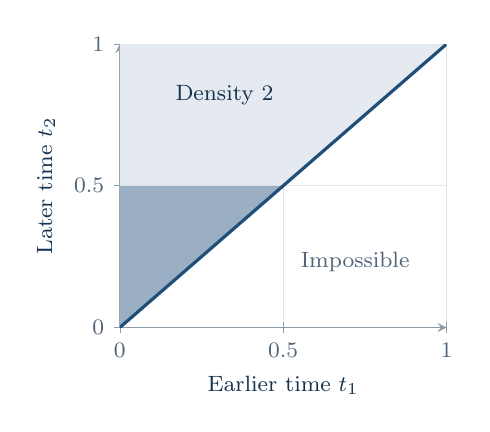
\begin{tikzpicture}
\begin{axis}[lecture square,width=4.15cm,height=3.6cm,
  xmin=0,xmax=1,ymin=0,ymax=1,
  xtick={0,0.5,1},ytick={0,0.5,1},
  xlabel={Earlier time $t_1$},ylabel={Later time $t_2$}]
  \path[fill=Blue!12,draw=none]
    (axis cs:0,0) -- (axis cs:0,1) -- (axis cs:1,1) -- cycle;
  \path[fill=Blue!45,draw=none]
    (axis cs:0,0) -- (axis cs:0,0.5) -- (axis cs:0.5,0.5) -- cycle;
  \addplot[Blue] coordinates {(0,0) (1,1)};
  \node[font=\footnotesize,text=Ink] at (axis cs:0.32,0.82) {Density $2$};
  \node[font=\footnotesize,text=Muted] at (axis cs:0.72,0.23) {Impossible};
\end{axis}
\end{tikzpicture}%
}

\newcommand{\ArrivalMarginalsPlot}{%
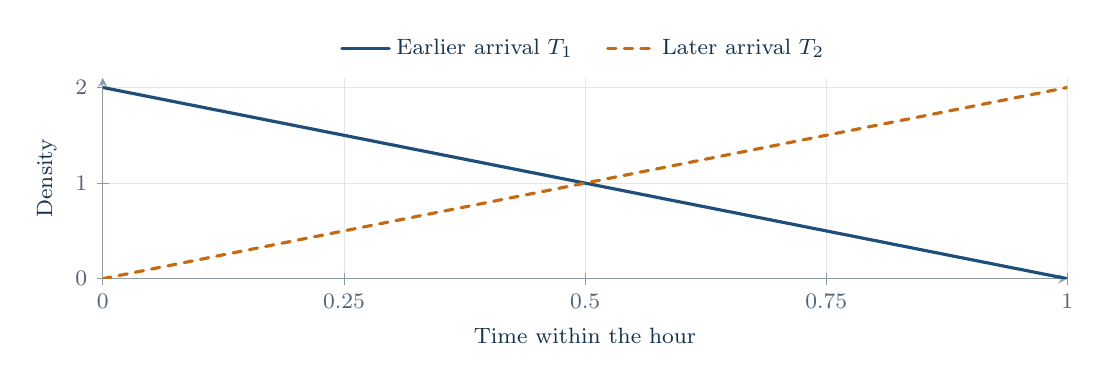
\begin{tikzpicture}
\begin{axis}[lecture wide,height=2.55cm,
  xmin=0,xmax=1,ymin=0,ymax=2.1,
  xlabel={Time within the hour},ylabel={Density},
  xtick={0,0.25,0.5,0.75,1},ytick={0,1,2},legend columns=2,
  domain=0:1,samples=2]
  \addplot[Blue] {2*(1-x)};
  \addlegendentry{Earlier arrival $T_1$}
  \addplot[Orange,dashed] {2*x};
  \addlegendentry{Later arrival $T_2$}
\end{axis}
\end{tikzpicture}%
}

\newcommand{\ConditionalArrivalPlot}{%
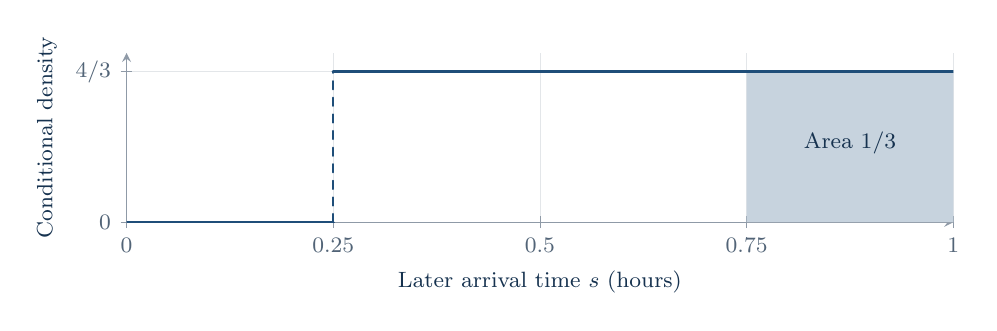
\begin{tikzpicture}
\begin{axis}[lecture axis,width=10.5cm,height=2.15cm,
  xmin=0,xmax=1,ymin=0,ymax=1.5,
  xtick={0,0.25,0.5,0.75,1},ytick={0,1.333333},yticklabels={$0$,$4/3$},
  xlabel={Later arrival time $s$ (hours)},ylabel={Conditional density}]
  \addplot[fill=Blue!25,draw=none]
    coordinates {(0.75,0) (0.75,1.333333) (1,1.333333) (1,0)} \closedcycle;
  \addplot[Blue] coordinates {(0,0) (0.25,0)};
  \addplot[Blue,dashed,line width=0.7pt] coordinates {(0.25,0) (0.25,1.333333)};
  \addplot[Blue] coordinates {(0.25,1.333333) (1,1.333333)};
  \node[font=\footnotesize,text=Ink] at (axis cs:0.875,0.7) {Area $1/3$};
\end{axis}
\end{tikzpicture}%
}

\newcommand{\NonlinearPlot}{%
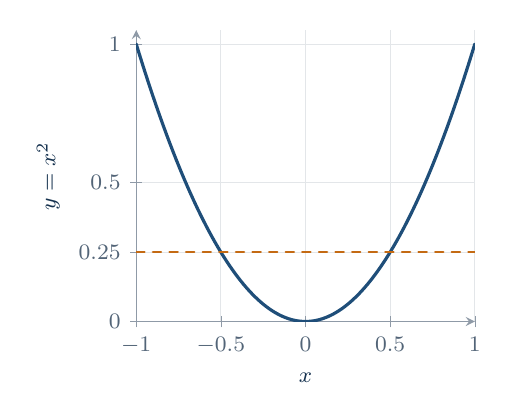
\begin{tikzpicture}
\begin{axis}[lecture square,
  xmin=-1,xmax=1,ymin=0,ymax=1.05,
  xtick={-1,-0.5,0,0.5,1},ytick={0,0.25,0.5,1},
  xlabel={$x$},ylabel={$y=x^2$},domain=-1:1,samples=121]
  \addplot[Blue] {x^2};
  \addplot[Orange,dashed,line width=0.8pt] coordinates {(-1,0.25) (1,0.25)};
\end{axis}
\end{tikzpicture}%
}

% The image of a radius-r circle under (z1,z2) -> (z1,rho*z1+sqrt(1-rho^2)*z2)
% is exactly the contour with squared Mahalanobis distance r^2.
\newcommand{\CorrelationContoursPlot}{%
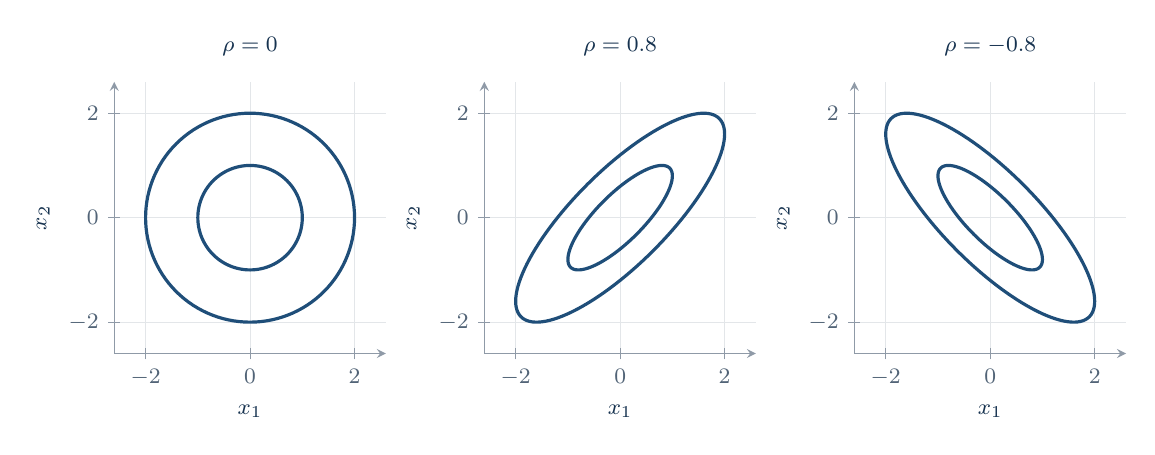
\begin{tikzpicture}
\begin{groupplot}[lecture axis,width=3.45cm,height=3.45cm,
  group style={group size=3 by 1,horizontal sep=1.25cm},
  xmin=-2.6,xmax=2.6,ymin=-2.6,ymax=2.6,
  xtick={-2,0,2},ytick={-2,0,2},xlabel={$x_1$},ylabel={$x_2$},
  domain=0:360,samples=121]
\nextgroupplot[title={$\rho=0$}]
  \addplot[Blue] ({cos(x)},{sin(x)});
  \addplot[Blue] ({2*cos(x)},{2*sin(x)});
\nextgroupplot[title={$\rho=0.8$}]
  \addplot[Blue] ({cos(x)},{0.8*cos(x)+0.6*sin(x)});
  \addplot[Blue] ({2*cos(x)},{2*(0.8*cos(x)+0.6*sin(x))});
\nextgroupplot[title={$\rho=-0.8$}]
  \addplot[Blue] ({cos(x)},{-0.8*cos(x)+0.6*sin(x)});
  \addplot[Blue] ({2*cos(x)},{2*(-0.8*cos(x)+0.6*sin(x))});
\end{groupplot}
\end{tikzpicture}%
}

\newcommand{\MahalanobisPlot}{%
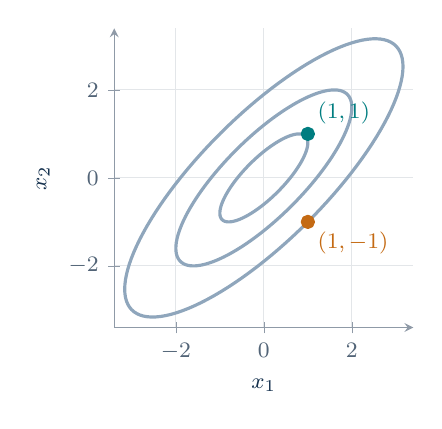
\begin{tikzpicture}
\begin{axis}[lecture square,width=3.8cm,height=3.8cm,
  xmin=-3.4,xmax=3.4,ymin=-3.4,ymax=3.4,
  xtick={-2,0,2},ytick={-2,0,2},xlabel={$x_1$},ylabel={$x_2$},
  domain=0:360,samples=121]
  \addplot[Blue!50] ({cos(x)},{0.8*cos(x)+0.6*sin(x)});
  \addplot[Blue!50] ({2*cos(x)},{2*(0.8*cos(x)+0.6*sin(x))});
  \addplot[Blue!50] ({sqrt(10)*cos(x)},{sqrt(10)*(0.8*cos(x)+0.6*sin(x))});
  \addplot[Teal,only marks,mark=*,mark size=2pt] coordinates {(1,1)};
  \addplot[Orange,only marks,mark=*,mark size=2pt] coordinates {(1,-1)};
  \node[font=\footnotesize,text=Teal,anchor=south west] at (axis cs:1,1) {$(1,1)$};
  \node[font=\footnotesize,text=Orange,anchor=north west] at (axis cs:1,-1) {$(1,-1)$};
\end{axis}
\end{tikzpicture}%
}

\newcommand{\RandomSignPlot}{%
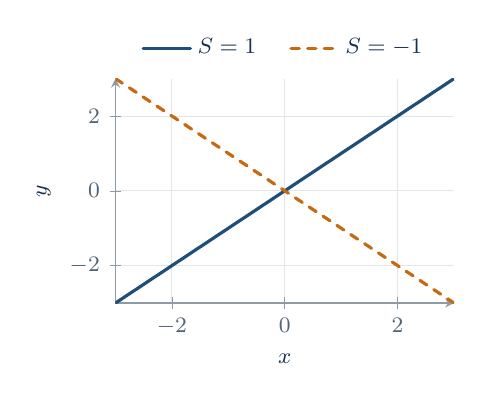
\begin{tikzpicture}
\begin{axis}[lecture square,height=2.85cm,legend columns=2,
  xmin=-3,xmax=3,ymin=-3,ymax=3,
  xtick={-2,0,2},ytick={-2,0,2},xlabel={$x$},ylabel={$y$},
  domain=-3:3,samples=2]
  \addplot[Blue] {x};
  \addlegendentry{$S=1$}
  \addplot[Orange,dashed] {-x};
  \addlegendentry{$S=-1$}
\end{axis}
\end{tikzpicture}%
}

\newcommand{\ConditionalDensityPlot}{%
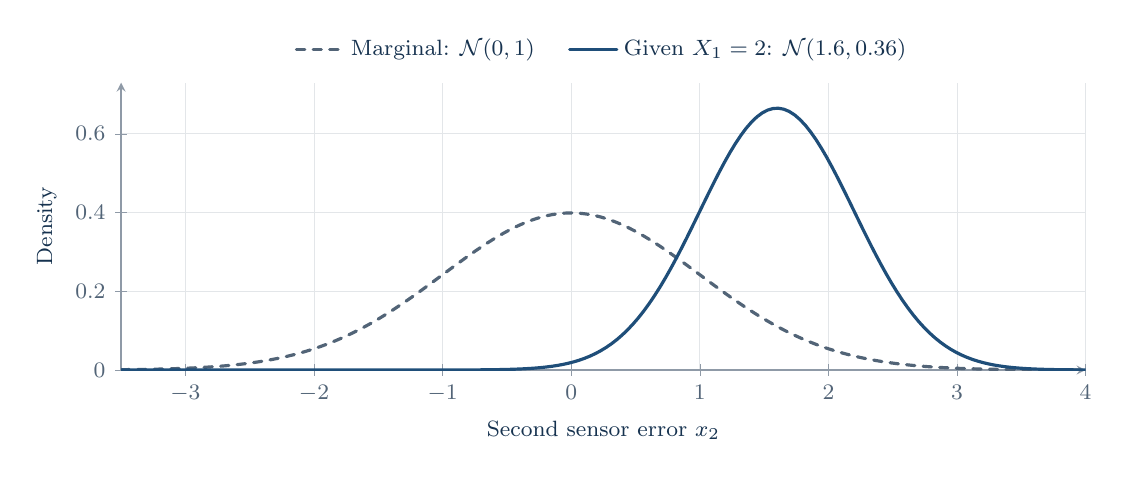
\begin{tikzpicture}
\begin{axis}[lecture wide,
  xmin=-3.5,xmax=4,ymin=0,ymax=0.73,
  xtick={-3,-2,-1,0,1,2,3,4},ytick={0,0.2,0.4,0.6},
  xlabel={Second sensor error $x_2$},ylabel={Density},
  domain=-3.5:4,samples=180,legend columns=2]
  \addplot[Muted,dashed] {exp(-x^2/2)/sqrt(2*pi)};
  \addlegendentry{Marginal: $\mathcal N(0,1)$}
  \addplot[Blue] {exp(-(x-1.6)^2/(2*0.36))/(0.6*sqrt(2*pi))};
  \addlegendentry{Given $X_1=2$: $\mathcal N(1.6,0.36)$}
\end{axis}
\end{tikzpicture}%
}

\newcommand{\ClassContoursPlot}{%
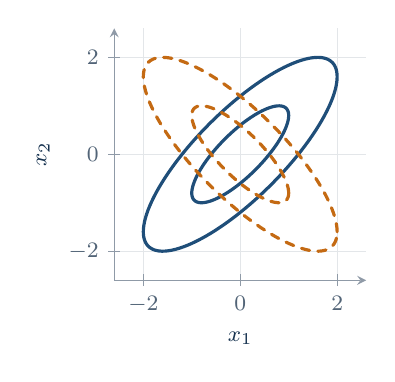
\begin{tikzpicture}
\begin{axis}[lecture square,width=3.2cm,height=3.2cm,
  xmin=-2.6,xmax=2.6,ymin=-2.6,ymax=2.6,
  xtick={-2,0,2},ytick={-2,0,2},xlabel={$x_1$},ylabel={$x_2$},
  domain=0:360,samples=121]
  \addplot[Blue] ({cos(x)},{0.8*cos(x)+0.6*sin(x)});
  \addplot[Blue] ({2*cos(x)},{2*(0.8*cos(x)+0.6*sin(x))});
  \addplot[Orange,dashed] ({cos(x)},{-0.8*cos(x)+0.6*sin(x)});
  \addplot[Orange,dashed] ({2*cos(x)},{2*(-0.8*cos(x)+0.6*sin(x))});
\end{axis}
\end{tikzpicture}%
}


\title{Joint distributions, dependence,\texorpdfstring{\\}{ }and random vectors}
\subtitle{Lecture 3}
\author{}
\date{Scientific Computing 2026}
\hypersetup{pdftitle={Lecture 3: Joint distributions, dependence, and random vectors},
  pdfsubject={Scientific Computing 2026, Chapter 3},pdfauthor={}}

\begin{document}

{\setbeamercolor{background canvas}{bg=Ink}
\begin{frame}[plain]
  \color{white}
  {\large Scientific Computing 2026\par}
  \vfill
  {\LARGE\bfseries Joint distributions, dependence,\\[0.2em]
    and random vectors\par}
  \vfill
  {\large Lecture 3\par}
  \vspace{4mm}
\end{frame}}

\begin{frame}{Two responses from the same user}
One user has click probability $P=0.1$ or $0.9$, equally likely.\\
Given $P$, the responses $X,Y\in\{0,1\}$ are independent.
\begin{definitionbox}{Joint probability mass function}
\blockmath{p_{X,Y}(x,y)=\Prob(X=x,Y=y)}
\end{definitionbox}
\vfill
\centering
\renewcommand{\arraystretch}{1.12}
\begin{tabular}{@{}lccc@{}}
\toprule
 & $Y=0$ & $Y=1$ & Total\\
\midrule
$X=0$ & $0.41$ & $0.09$ & $0.50$\\
$X=1$ & $0.09$ & $0.41$ & $0.50$\\
\midrule
Total & $0.50$ & $0.50$ & $1$\\
\bottomrule
\end{tabular}
\par
\takeaway{$p_{X,Y}(1,1)=\tfrac12(0.1)^2+\tfrac12(0.9)^2=0.41$.}
\end{frame}

\begin{frame}{Marginals discard the pairing}
\begin{definitionbox}{Marginal PMFs}
\blockmath{p_X(x)=\sum_y p_{X,Y}(x,y),\qquad
  p_Y(y)=\sum_x p_{X,Y}(x,y)}
\end{definitionbox}
\vfill
\begin{columns}[T,onlytextwidth]
\begin{column}{0.47\textwidth}
\textbf{Same user}
\[
  (p_{X,Y}(x,y))=
  \begin{pmatrix}0.41&0.09\\0.09&0.41\end{pmatrix}
\]
Agreement is more likely.
\end{column}
\begin{column}{0.47\textwidth}
\textbf{Independently selected users}
\[
  (p_{X,Y}(x,y))=
  \begin{pmatrix}0.25&0.25\\0.25&0.25\end{pmatrix}
\]
All pairs are equally likely.
\end{column}
\end{columns}
\takeaway{Both models have $X,Y\sim\operatorname{Bernoulli}(0.5)$.
The marginals do not determine the joint distribution.}
\end{frame}

\begin{frame}{A conditional PMF normalizes one row}
For the same user,
\[
  \Prob(Y=1\mid X=1)=\frac{0.41}{0.50}=0.82,\qquad
  \Prob(Y=1\mid X=0)=\frac{0.09}{0.50}=0.18.
\]
\vfill
\begin{definitionbox}{Conditional PMF}
For $p_X(x)>0$,
\[
  p_{Y\mid X}(y\mid x)=\frac{p_{X,Y}(x,y)}{p_X(x)}.
\]
\end{definitionbox}
\vfill
Rearranging gives the factorization
\[
  p_{X,Y}(x,y)=p_X(x)\,p_{Y\mid X}(y\mid x).
\]
\end{frame}

\begin{frame}{Independence depends on what we condition on}
Independence requires
\[
  p_{X,Y}(x,y)=p_X(x)p_Y(y)\qquad\text{for every }x,y.
\]
The shared-user table fails: $0.41\ne0.5\cdot0.5$.
\vfill
\begin{definitionbox}{Conditional independence given $P$}
Within each user type, the joint PMF factors:
\[
  p_{X,Y\mid P}(x,y\mid p)
  =p_{X\mid P}(x\mid p)\,p_{Y\mid P}(y\mid p).
\]
\end{definitionbox}
\takeaway{The first click provides information about the user's probability $P$.
This does not mean that one click causes the other.}
\end{frame}

\renewcommand{\conspectsection}{3.2}
\begin{frame}{Joint densities assign probability to regions}
Near $(x,y)$, a small rectangle has probability approximately
\[
  f_{X,Y}(x,y)\,\Delta x\,\Delta y.
\]
\vfill
\begin{definitionbox}{Joint density}
A nonnegative function with total integral one, satisfying
\[
  \Prob((X,Y)\in R)=\iint_R f_{X,Y}(x,y)\,dx\,dy
\]
for regions $R$ in the plane.
\end{definitionbox}
\takeaway{Integrating over a region adds the probabilities of its small rectangles.}
\end{frame}

\begin{frame}{Two arrivals, recorded in order}
Independent $U,V\sim\operatorname{Uniform}(0,1)$, in hours.\\
Record $T_1=\min(U,V)$ and $T_2=\max(U,V)$.
\vfill
\begin{columns}[c,onlytextwidth]
\begin{column}{0.45\textwidth}
\centering\ArrivalRegionPlot
\end{column}
\begin{column}{0.52\textwidth}
Either person can arrive first:
\[
  f_{T_1,T_2}(t,s)=2,\quad 0<t<s<1.
\]
Density is zero elsewhere.
\medskip
Both arrive before half an hour:
\[
  \Prob(T_2\le\tfrac12)
  =2\cdot\frac18=\frac14.
\]
\end{column}
\end{columns}
\takeaway{Sorting introduces dependence: the later arrival must follow the earlier one.}
\end{frame}

\begin{frame}{Marginals integrate over the other arrival}
\centering\ArrivalMarginalsPlot
\par
\blockmath{
  f_{T_1}(t)=\int_t^1 2\,ds=2(1-t),\qquad
  f_{T_2}(s)=\int_0^s 2\,dt=2s.}
\takeaway{An early first arrival leaves more possible times for the second.
In general, $f_X(x)=\int_{\Real}f_{X,Y}(x,y)\,dy$.}
\end{frame}

\begin{frame}{A conditional density normalizes one slice}
Given $T_1=t$, the later arrival can be anywhere in $(t,1)$.
\begin{definitionbox}{Conditional density}
Where $f_X(x)>0$,
\[
  f_{Y\mid X}(y\mid x)=\frac{f_{X,Y}(x,y)}{f_X(x)}.
\]
\end{definitionbox}
\[
  f_{T_2\mid T_1}(s\mid t)=\frac{2}{2(1-t)}=\frac1{1-t},
  \quad t<s<1.
\]
\takeaway{For smooth densities, this is the limit of conditioning on a small
interval around $x$. The denominator is a density.}
\end{frame}

\begin{frame}{Conditional probability of a late second arrival}
The first arrival is at $t=\tfrac14$. The second is uniform over
the remaining $\tfrac34$ hour.
\vfill
\centering\ConditionalArrivalPlot
\par
\blockmath{\Prob(T_2>\tfrac34\mid T_1=\tfrac14)
  =\int_{3/4}^1\frac43\,ds=\frac13.}
\takeaway{The shaded area is the probability that the second arrival occurs
in the final quarter-hour, given the first arrival at 15 minutes.}
\end{frame}

\begin{frame}{The expected gap between arrivals}
The expectation rule now uses the joint density:
\[
  \Expect[g(X,Y)]=\iint_{\Real^2}g(x,y)f_{X,Y}(x,y)\,dx\,dy.
\]
\vfill
For the gap $g(t,s)=s-t$,
\begin{align*}
  \Expect[T_2-T_1]
  &=\int_0^1\int_t^1 (s-t)\,2\,ds\,dt\\[0.4em]
  &=\int_0^1(1-t)^2\,dt=\frac13\text{ hour}.
\end{align*}
\takeaway{For a discrete pair, replace the integrals by sums.
A finite expectation requires $\Expect[|g(X,Y)|]<\infty$.}
\end{frame}

\renewcommand{\conspectsection}{3.3}
\begin{frame}{Correlation removes the units}
For the click table,
\[
  \Cov(X,Y)=\Expect[XY]-\Expect[X]\Expect[Y]
  =0.41-0.25=0.16.
\]
\begin{definitionbox}{Correlation}
For finite, positive standard deviations $\sigma_X,\sigma_Y$,
\[
  \rho_{X,Y}=\frac{\Cov(X,Y)}{\sigma_X\sigma_Y}
  =\Expect\!\left[
    \frac{X-\mu_X}{\sigma_X}\frac{Y-\mu_Y}{\sigma_Y}\right].
\]
\end{definitionbox}
\vfill
For the clicks, $\sigma_X=\sigma_Y=0.5$, so $\rho_{X,Y}=0.64$.
\takeaway{Changing minutes to seconds changes covariance but leaves correlation unchanged.}
\end{frame}

\begin{frame}{Why correlation lies between $-1$ and $1$}
Standardize: $U=(X-\mu_X)/\sigma_X$, $V=(Y-\mu_Y)/\sigma_Y$.
\[
  0\le\Expect[(U-V)^2]=2-2\rho,\qquad
  0\le\Expect[(U+V)^2]=2+2\rho.
\]
\begin{resultbox}{Correlation bound and equality cases}
For finite, positive marginal variances, $-1\le\rho\le1$.
\[
  \rho=1\ \Longleftrightarrow\ U=V\text{ almost surely},\qquad
  \rho=-1\ \Longleftrightarrow\ U=-V\text{ almost surely}.
\]
\end{resultbox}
\vfill
Perfect correlation means an exact affine relationship.
\takeaway{If either variable is constant, correlation is undefined.}
\end{frame}

\begin{frame}{Zero correlation can hide complete dependence}
Let $X\sim\operatorname{Uniform}(-1,1)$ and $Y=X^2$.
\vfill
\begin{columns}[c,onlytextwidth]
\begin{column}{0.47\textwidth}
\centering\NonlinearPlot
\end{column}
\begin{column}{0.49\textwidth}
Symmetry gives
\[
  \Expect[X]=\Expect[X^3]=0.
\]
Therefore
\[
  \Cov(X,Y)=0,\qquad\rho_{X,Y}=0.
\]
Yet knowing $X$ determines $Y$ exactly.
\end{column}
\end{columns}
\takeaway{$\Prob(Y\le1/4\mid |X|\le1/2)=1$, while
$\Prob(Y\le1/4)=1/2$. Independence fails.}
\end{frame}

\renewcommand{\conspectsection}{3.4}
\begin{frame}{Conditional means minimize squared prediction error}
Use $X$ to predict $Y$. Write
\[
  m(x)=\Expect[Y\mid X=x],\qquad v(x)=\Var(Y\mid X=x).
\]
\begin{theorembox}{Best prediction under squared error}
If $\Expect[Y^2]<\infty$, every rule $a(X)$ with finite mean squared
error satisfies
\[
  \Expect[(Y-a(X))^2]
  =\Expect[v(X)]+\Expect[(m(X)-a(X))^2].
\]
The minimum is $\Expect[v(X)]$, attained by $a(X)=m(X)$.
\end{theorembox}
\takeaway{The two terms are remaining uncertainty and the extra error from using a different prediction.}
\end{frame}

\begin{frame}{Why the conditional mean is optimal}
Inside the group $X=x$, split the prediction error:
\[
  Y-a(x)=(Y-m(x))+(m(x)-a(x)).
\]
The cross term averages to zero because
\[
  \Expect[Y-m(x)\mid X=x]=0.
\]
\vfill
Squaring and taking conditional expectation gives
\[
  \Expect[(Y-a(x))^2\mid X=x]=v(x)+(m(x)-a(x))^2.
\]
\takeaway{Total expectation averages this identity over $X$.}
\end{frame}

\begin{frame}{Prediction in the click model}
Without the first response, the best constant prediction is $0.5$.
\[
  \Expect[(Y-0.5)^2]=0.25.
\]
\vfill
After observing it,
\[
  m(0)=0.18,\qquad m(1)=0.82.
\]
Both groups have the same conditional variance:
\focusmath{\Expect[(Y-m(X))^2]=0.18(0.82)=0.1476.}
\takeaway{These are predictions from a specified probability model.
Learning the rule from data is a separate estimation problem.}
\end{frame}

\renewcommand{\conspectsection}{3.5}
\begin{frame}{Several measurements on one object}
Record several sensor readings, or several features of one observation.
\begin{definitionbox}{Random vector and mean vector}
\blockmath{\mathbf X=
  \begin{pmatrix}X_1\\\vdots\\X_d\end{pmatrix}\in\Real^d,
  \qquad
  \boldsymbol\mu=\Expect[\mathbf X]=
  \begin{pmatrix}\Expect[X_1]\\\vdots\\\Expect[X_d]\end{pmatrix}}
\end{definitionbox}
\vfill
All coordinates belong to the same object or experimental repetition.\\
A realized observation is a lowercase vector $\mathbf x$.
\takeaway{The joint distribution assigns probabilities to regions in $\Real^d$.}
\end{frame}

\begin{frame}{A covariance matrix records every pair}
\begin{definitionbox}{Covariance matrix}
For a random vector with finite second moments,
\[
  \Sigma=\Expect[(\mathbf X-\boldsymbol\mu)
    (\mathbf X-\boldsymbol\mu)^\top],\qquad
  \Sigma_{ij}=\Cov(X_i,X_j).
\]
\end{definitionbox}
Diagonal entries are variances. Off-diagonal entries are covariances.
\vfill
For the two clicks,
\[
  \boldsymbol\mu=\begin{pmatrix}0.5\\0.5\end{pmatrix},\qquad
  \Sigma=\begin{pmatrix}0.25&0.16\\0.16&0.25\end{pmatrix}.
\]
\takeaway{Standardizing the coordinates gives $R_{ij}=\Sigma_{ij}/
\sqrt{\Sigma_{ii}\Sigma_{jj}}$. Here $R$ has diagonal $1$ and off-diagonal $0.64$.}
\end{frame}

\begin{frame}{Every weighted sum must have nonnegative variance}
For $S=\mathbf a^\top\mathbf X=\sum_i a_iX_i$,
\[
  \Var(S)=\sum_i\sum_j a_i a_j\Sigma_{ij}
  =\mathbf a^\top\Sigma\mathbf a\ge0.
\]
\begin{definitionbox}{Positive semidefinite matrix}
A symmetric matrix $\Sigma$ is positive semidefinite when
\[
  \mathbf a^\top\Sigma\mathbf a\ge0\qquad\text{for every real }\mathbf a.
\]
It is positive definite when this is strictly positive for every
nonzero $\mathbf a$.
\end{definitionbox}
\takeaway{Every covariance matrix is positive semidefinite.
A zero-variance combination can make it singular.}
\end{frame}

\begin{frame}{Positive diagonal entries are not enough}
Could this be a covariance matrix?
\[
  M=\begin{pmatrix}1&2\\2&1\end{pmatrix}
\]
It would imply
\[
  \Var(X_1-X_2)=1+1-2(2)=-2.
\]
\begin{resultbox}{Valid covariance matrices in two dimensions}
\blockmath{\begin{pmatrix}v_1&c\\c&v_2\end{pmatrix}\succeq0
  \quad\Longleftrightarrow\quad
  v_1\ge0,\quad v_2\ge0,\quad c^2\le v_1v_2}
\end{resultbox}
\takeaway{With positive variances, the last condition is exactly $|\rho|\le1$.
A diagonal covariance matrix alone does not guarantee independence.}
\end{frame}

\renewcommand{\conspectsection}{3.6}
\begin{frame}{Means and covariances after a linear transformation}
Let $\mathbf W=A\mathbf X+\mathbf b$, with fixed $A$ and $\mathbf b$.
\begin{theorembox}{Linear transformation of moments}
For $\Expect[\mathbf X]=\boldsymbol\mu$ and finite covariance $\Sigma$,
\[
  \Expect[\mathbf W]=A\boldsymbol\mu+\mathbf b,\qquad
  \Cov(\mathbf W)=A\Sigma A^\top.
\]
\end{theorembox}
\vfill
\textbf{Proof.} Centering removes the shift:
\[
  \mathbf W-\Expect[\mathbf W]=A(\mathbf X-\boldsymbol\mu).
\]
Take the expected outer product and pull out the fixed matrices.
\takeaway{These rules need neither independence nor a Gaussian distribution.}
\end{frame}

\begin{frame}{Average error and disagreement between sensors}
Centered errors have $\Sigma=\begin{pmatrix}1&0.8\\0.8&1\end{pmatrix}$.
\[
  M=\frac{X_1+X_2}{2},\quad D=X_1-X_2,\quad
  A=\begin{pmatrix}1/2&1/2\\1&-1\end{pmatrix}.
\]
\[
  \Cov\!\begin{pmatrix}M\\D\end{pmatrix}
  =A\Sigma A^\top=\begin{pmatrix}0.9&0\\0&0.4\end{pmatrix}.
\]
\vfill
Averaging retains much of the shared error.\\
Taking the difference cancels much of it.
\takeaway{With independent unit-variance errors, the variances would be $0.5$ and $2$.
Zero covariance between $M$ and $D$ does not yet establish independence.}
\end{frame}

\renewcommand{\conspectsection}{3.7}
\begin{frame}{Correlated Gaussian readings from independent noise}
Take independent $Z_1,Z_2\sim\mathcal N(0,1)$ and set
\focusmath{X_1=Z_1,\qquad X_2=0.8Z_1+0.6Z_2.}
Both sensors contain the disturbance $Z_1$.\\
Only the second contains the additional disturbance $Z_2$.
\vfill
\[
  \Var(X_2)=0.8^2+0.6^2=1,\qquad
  \Cov(X_1,X_2)=0.8.
\]
\takeaway{Both marginals are standard Gaussian.
Their joint distribution records the shared noise.}
\end{frame}

\begin{frame}{The multivariate Gaussian construction}
\begin{definitionbox}{Multivariate Gaussian}
Let $\mathbf Z$ have independent standard Gaussian coordinates.
For fixed $A$ and $\boldsymbol\mu$,
\[
  \mathbf X=\boldsymbol\mu+A\mathbf Z
  \sim\mathcal N_d(\boldsymbol\mu,\Sigma),\qquad\Sigma=AA^\top.
\]
\end{definitionbox}
\vfill
Every linear combination is Gaussian:
\[
  \mathbf a^\top\mathbf X\sim
  \mathcal N(\mathbf a^\top\boldsymbol\mu,
    \mathbf a^\top\Sigma\mathbf a).
\]
\takeaway{Zero variance means a constant.
The rows of $A$ specify which independent noises each measurement shares.}
\end{frame}

\begin{frame}{Correlation changes the joint shape}
\centering\CorrelationContoursPlot
\plotcaption{In every panel, both marginals are $\mathcal N(0,1)$.
Each curve joins points of equal density. Outer curves have lower density.}
\end{frame}

\begin{frame}{The bivariate density from a change of coordinates}
For $|\rho|<1$, write
\[
  X_1=Z_1,\qquad X_2=\rho Z_1+\sqrt{1-\rho^2}\,Z_2.
\]
The inverse uses $z_1=x_1$, $z_2=(x_2-\rho x_1)/\sqrt{1-\rho^2}$.
The transformation multiplies areas by $\sqrt{1-\rho^2}$.
\vfill
\begin{resultbox}{Standard bivariate Gaussian density}
\blockmath{f(x_1,x_2)=\frac1{2\pi\sqrt{1-\rho^2}}
  \exp\!\left[-\frac{x_1^2-2\rho x_1x_2+x_2^2}{2(1-\rho^2)}\right]}
\end{resultbox}
\takeaway{Substitute the inverse into the independent-noise density
and divide by the area scale to preserve probability.}
\end{frame}

\begin{frame}{The long and short directions of a Gaussian ellipse}
For $\rho=0.8$, use rotated coordinates
\[
  U=\frac{X_1+X_2}{\sqrt2},\qquad
  V=\frac{X_1-X_2}{\sqrt2}.
\]
Their variances are $1.8$ and $0.2$, with covariance zero.
\vfill
The exponent depends on
\focusmath{q=\frac{u^2}{1.8}+\frac{v^2}{0.2}.}
At $q=c$, the axis lengths are proportional to
$\sqrt{1.8c}$ and $\sqrt{0.2c}$.
\takeaway{The equal-sign direction is three times longer.
Shared sensor fluctuations stretch the distribution along the diagonal.}
\end{frame}

\begin{frame}{The Gaussian density in matrix notation}
\begin{resultbox}{Multivariate Gaussian density}
For a positive-definite covariance matrix $\Sigma$,
\[
  f_{\mathbf X}(\mathbf x)=
  \frac{\exp[-\tfrac12 q(\mathbf x)]}
       {(2\pi)^{d/2}\sqrt{\det\Sigma}},
  \qquad
  q(\mathbf x)=(\mathbf x-\boldsymbol\mu)^\top
  \Sigma^{-1}(\mathbf x-\boldsymbol\mu).
\]
\end{resultbox}
\vfill
$q(\mathbf x)$ is the sum of squared independent-noise coordinates.\\
$\sqrt{\det\Sigma}$ accounts for the change in volume.
\takeaway{$\Sigma^{-1}$ is the inverse and $\det\Sigma$ the determinant.
For diagonal $\Sigma$, the density factors into univariate Gaussian densities.}
\end{frame}

\begin{frame}{Equal ordinary distance, different Gaussian density}
\begin{columns}[c,onlytextwidth]
\begin{column}{0.46\textwidth}
\centering\MahalanobisPlot
\end{column}
\begin{column}{0.50\textwidth}
For unit variances and $\rho=0.8$,
\[
  q(1,1)=\frac{10}{9},\qquad q(1,-1)=10.
\]
Both points are distance $\sqrt2$ from the origin.
\medskip
The disagreement $(1,-1)$ has much lower density.
\end{column}
\end{columns}
\begin{definitionbox}{Squared Mahalanobis distance}
\blockmath{q(\mathbf x)=(\mathbf x-\boldsymbol\mu)^\top
  \Sigma^{-1}(\mathbf x-\boldsymbol\mu)}
\end{definitionbox}
\end{frame}

\begin{frame}{Gaussian transformations and independence}
\begin{theorembox}{Closure under linear transformations}
If $\mathbf X\sim\mathcal N_d(\boldsymbol\mu,\Sigma)$, then for fixed $B,\mathbf b$,
\[
  B\mathbf X+\mathbf b\sim
  \mathcal N(B\boldsymbol\mu+\mathbf b,\,B\Sigma B^\top).
\]
\end{theorembox}
Selecting coordinates gives Gaussian marginals.
\vfill
\begin{theorembox}{The joint Gaussian independence exception}
For jointly Gaussian variables, zero covariance implies independence.
\end{theorembox}
\takeaway{Thus the sensor average and difference are independent under the joint
Gaussian model. The moment rules now specify their full distribution.}
\end{frame}

\begin{frame}{Gaussian marginals do not guarantee a joint Gaussian}
Take $X\sim\mathcal N(0,1)$ and an independent random sign $S=\pm1$,
each with probability $1/2$. Set $Y=SX$.
\vfill
\begin{columns}[c,onlytextwidth]
\begin{column}{0.46\textwidth}
\centering\RandomSignPlot
\end{column}
\begin{column}{0.50\textwidth}
$Y\sim\mathcal N(0,1)$, and
\[
  \Cov(X,Y)=\Expect[SX^2]=0.
\]
But $|Y|=|X|$ always.\\
The variables are dependent.
\medskip
$X+Y$ equals zero with probability $1/2$, but is not constant.
\end{column}
\end{columns}
\takeaway{A joint Gaussian would make every linear combination Gaussian.
This one has a point mass, so the pair is not jointly Gaussian.}
\end{frame}

\begin{frame}{A singular Gaussian lives on a lower-dimensional set}
Let $X_2=X_1\sim\mathcal N(0,1)$.
\[
  \Sigma=\begin{pmatrix}1&1\\1&1\end{pmatrix},\qquad
  \det\Sigma=0,\qquad\Var(X_1-X_2)=0.
\]
\vfill
Every observation lies on the line $x_2=x_1$.
\vfill
This is a valid Gaussian random vector, but it has no density
with respect to two-dimensional area.
\takeaway{The Gaussian construction allows singular covariance matrices.
The full-dimensional density formula requires positive definiteness.}
\end{frame}

\renewcommand{\conspectsection}{3.8}
\begin{frame}{Observing one sensor reveals the shared noise}
Recall the construction
\[
  X_1=Z_1,\qquad X_2=0.8Z_1+0.6Z_2.
\]
Observing $X_1=x$ fixes $Z_1=x$. Only $Z_2$ remains random.
\focusmath{X_2\mid X_1=x\sim\mathcal N(0.8x,0.36).}
\vfill
If the first sensor reads two units too high, the second has
conditional mean $1.6$ and conditional standard deviation $0.6$.
\takeaway{The marginal distribution of $X_2$ remains $\mathcal N(0,1)$.}
\end{frame}

\begin{frame}{Conditioning shifts the mean and reduces the spread}
\centering\ConditionalDensityPlot
\plotcaption{At $X_1=2$, the second sensor's mean shifts from $0$ to $1.6$.
Its variance falls from $1$ to $0.36$.}
\end{frame}

\begin{frame}{The general conditional Gaussian formula}
\begin{theorembox}{Conditioning a bivariate Gaussian}
For jointly Gaussian $X,Y$ with $\sigma_X,\sigma_Y>0$ and $|\rho|<1$,
\[
  Y\mid X=x\sim\mathcal N\!\left(
    \mu_Y+\rho\frac{\sigma_Y}{\sigma_X}(x-\mu_X),\,
    \sigma_Y^2(1-\rho^2)\right).
\]
\end{theorembox}
The mean's slope is $\Cov(X,Y)/\Var(X)$.\\
The conditional variance is constant in $x$ in this model.
\vfill
For the sensors, total variance gives
\blockmath{
  \underbrace{1}_{\text{total variance}}
  \qquad=\qquad\underbrace{0.36}_{\text{residual variance}}
  \qquad+\qquad\underbrace{0.64}_{\text{variance of conditional mean}}.}
\takeaway{At $|\rho|=1$, the relationship is exact and the conditional distribution is a point mass.}
\end{frame}

\renewcommand{\conspectsection}{3.9}
\begin{frame}{Two operating modes with identical feature marginals}
Two equally likely modes, both with mean zero:
\[
  \Sigma_+=\begin{pmatrix}1&0.8\\0.8&1\end{pmatrix},\qquad
  \Sigma_-=\begin{pmatrix}1&-0.8\\-0.8&1\end{pmatrix}.
\]
\begin{columns}[c,onlytextwidth]
\begin{column}{0.46\textwidth}
\centering\ClassContoursPlot
\end{column}
\begin{column}{0.50\textwidth}
\textcolor{Blue}{Mode $+$}: errors move together.\\[0.6em]
\textcolor{Orange}{Mode $-$}: errors move in opposite directions.
\medskip
Each feature alone is $\mathcal N(0,1)$ in either class.
\end{column}
\end{columns}
\takeaway{The distinguishing information is entirely in the relationship between the features.}
\end{frame}

\begin{frame}{Agreement between features identifies the mode}
The determinants are equal, so the density normalization cancels:
\[
  \log\frac{f_+(x_1,x_2)}{f_-(x_1,x_2)}
  =\frac{2(0.8)}{1-0.8^2}\,x_1x_2=\frac{40}{9}x_1x_2.
\]
With equal priors, choose $+$ if $x_1x_2>0$, and $-$ if $x_1x_2<0$.
\vfill
At $(1,1)$,
\focusmath{\Prob(C=+\mid\mathbf X=(1,1))
  =\frac1{1+e^{-40/9}}\approx0.9884.}
At $(1,-1)$, the probability is approximately $0.0116$.
\takeaway{Along either coordinate axis the posterior probabilities tie.}
\end{frame}

\begin{frame}{An independence assumption can erase the signal}
Suppose we replace each class's joint density by the product
of its feature marginals.
\[
  \widetilde f_+(x_1,x_2)=\phi(x_1)\phi(x_2)
  =\widetilde f_-(x_1,x_2),
\]
where $\phi$ is the standard Gaussian density.
\vfill
Both approximate models now assign the same density to every pair.
\focusmath{\widetilde\Prob(C=+\mid\mathbf X=\mathbf x)=\frac12.}
\takeaway{Conditional independence within the class discards all of the
useful class information in this example.}
\end{frame}

\begin{frame}{The Gaussian classification score}
Model $\Prob(C=k)=\pi_k$ and
$\mathbf X\mid C=k\sim\mathcal N_d(\boldsymbol\mu_k,\Sigma_k)$.
\begin{resultbox}{Posterior-maximizing class score}
For $\pi_k>0$ and positive-definite $\Sigma_k$, choose the largest
\[
  s_k(\mathbf x)=\log\pi_k-\frac12\log\det\Sigma_k
  -\frac12(\mathbf x-\boldsymbol\mu_k)^\top
    \Sigma_k^{-1}(\mathbf x-\boldsymbol\mu_k).
\]
\end{resultbox}
\vfill
The terms account for class prevalence, density spread, and
displacement relative to the class covariance.
\takeaway{The omitted $-\tfrac d2\log(2\pi)$ is identical for every class.}
\end{frame}

\begin{frame}{Shared covariance gives linear decision boundaries}
If every class has the same covariance $\Sigma$, the quadratic term
$-\tfrac12\mathbf x^\top\Sigma^{-1}\mathbf x$ cancels in comparisons.
\vfill
The class-dependent score becomes
\[
  \mathbf x^\top\Sigma^{-1}\boldsymbol\mu_k
  -\frac12\boldsymbol\mu_k^\top\Sigma^{-1}\boldsymbol\mu_k
  +\log\pi_k.
\]
This is linear in the observed features, plus a constant.
\vfill
With different covariance matrices, quadratic terms generally remain.
The two-mode example uses the interaction $x_1x_2$.
\takeaway{Learning the means, covariances, and class probabilities from data
belongs to statistical estimation.}
\end{frame}

\begin{frame}{What the joint model lets us compute}
\renewcommand{\arraystretch}{1.5}
\begin{tabular}{@{}ll@{}}
\toprule
\textbf{Operation} & \textbf{What it answers}\\
\midrule
Marginalize & What remains if we ignore a measurement?\\
Condition & What changes after we observe a measurement?\\
Transform & How do combined measurements vary?\\
Compare class densities & Which class best explains the whole observation?\\
\bottomrule
\end{tabular}
\vfill
Dependence can matter even when each individual feature looks identical
across models.
\takeaway{Correlation summarizes linear dependence. A joint distribution can contain much more.}
\end{frame}

\end{document}
